\documentclass[conference]{IEEEtran}

\usepackage{amsmath}
\usepackage{amssymb}
\usepackage{graphicx}
\usepackage{booktabs}
\usepackage{tabularx}
\usepackage{tikz}
\usepackage{cite}
\usepackage{url}
\usepackage[hidelinks]{hyperref}
\usetikzlibrary{arrows.meta}

\title{Evidence-Driven Dataset Recommendation under Local Resource Constraints}

% Provisional author set and order; coauthor order, school wording, and the
% current status of the corresponding address are documented for confirmation.
\author{%
  \IEEEauthorblockN{%
    Pratham Kashyap\IEEEauthorrefmark{1},
    Anvesha Rastogi\IEEEauthorrefmark{1},
    Harsh Gupta\IEEEauthorrefmark{1},
    Harsh Dhoriyani\IEEEauthorrefmark{1},
    Priyanshu Ranjan\IEEEauthorrefmark{1}, and
    Shrish\IEEEauthorrefmark{1}%
  }
  \IEEEauthorblockA{%
    \IEEEauthorrefmark{1}School of Computing Science and Engineering, VIT Bhopal University, Sehore, India\\
    Corresponding author candidate: Pratham Kashyap,\ \texttt{pratham.23bai10455@vitbhopal.ac.in}%
  }
}

\begin{document}
\maketitle

\begin{abstract}
Dataset selection requires more than retrieving descriptions related to a query: task compatibility, provenance, content observations, and unresolved metadata must also be considered within practical resource limits. This paper describes an implemented, local-first dataset recommendation pipeline that accepts structured task specifications, records source claims and bounded observations in a two-layer evidence ledger, applies explicit compatibility gates, estimates task-specific utility, and emits provenance-linked recommendation cards. Candidate scoring combines fit, utility, evidence support, content coverage, and a risk penalty; a family-aware greedy selector then forms a compact set. Evaluation separates development experiments from a frozen offline benchmark of 24 dataset records and eight tasks. On that benchmark, the cumulative ablation reached mean set utility 0.8588, while the recorded run used 33.11 MiB peak memory and 327.49 ms with zero network egress; the robustness harness completed ten fixture-based trials without a crash. Diversification did not change mean utility in M8 because no qualifying same-family mirror pairs occurred in the realized candidate geometry. These results characterize the implemented system on the tested corpora; they do not establish web-scale effectiveness or downstream model gains. A three-participant card pilot is descriptive, and one registered hypothesis was not applicable.
\end{abstract}

\begin{IEEEkeywords}
Dataset recommendation, dataset provenance, task-specific utility, evidence representation, resource-constrained systems.
\end{IEEEkeywords}

\section{Introduction}
Selecting a dataset is an early modeling decision with consequences for what a machine-learning task can measure, which populations or conditions it represents, and whether its inputs and targets match the intended use. Public repositories and dataset-search services improve discovery across a distributed collection of sources~\cite{noy2019googledatasetsearch}. Systems such as DataFinder formalize dataset recommendation from natural-language descriptions and compare retrieval methods for identifying relevant candidates~\cite{viswanathan2023datafinder}. These systems address an important first step: finding datasets whose descriptions appear related to a research need.

Retrieval relevance, however, does not establish that a candidate is suitable for a particular task. A dataset description can suggest a matching domain while leaving unresolved whether its modality, target, label structure, access conditions, sample contents, or provenance satisfy the task's constraints. Nor should repository metadata automatically be treated as ground truth. Dataset descriptions are published claims; they may be absent, incomplete, inconsistent across sources, or contradicted by an accessible sample. A large-scale audit of dataset provenance and licensing reports substantial omissions and miscategorization in public dataset records~\cite{longpre2023dataprovenance}. That work motivates treating provenance and license fields as evidence to inspect, not as legal determinations. Structured metadata formats and dataset documentation improve description and communication, but the presence of a standard or card does not itself verify every claim against the underlying data~\cite{akhtar2024croissant,pushkarna2022datacards}.

Task-aware selection therefore calls for more than lexical or semantic similarity. It requires separating hard incompatibilities from soft preferences, recording what was observed versus asserted, and inspecting content when access permits. Such inspection must also be bounded: unrestricted downloads or large dense indexes may be infeasible in a local workflow. In this project, M0 established a 128~MiB process-memory ceiling from its measured resource profile, which constrained subsequent component choices. The engineering question is thus how to combine compatibility, task-specific utility estimates, provenance, and limited content evidence without implying that missing or unverified information is favorable.

This paper addresses a focused integration and evaluation problem. It presents an implemented pipeline that consumes structured task specifications, represents evidence using separate observation and resolution states, performs bounded sample fingerprinting, applies hard compatibility gates, estimates task utility with fixed heuristics, and selects a family-aware recommendation set with traceable cards. The implementation does not parse free-form requests, train a task-specific retriever, use formal Dempster--Shafer fusion, or claim downstream model-performance gains. Its scoring and selection mechanisms are integrations of established ideas; the contribution is their implementation and evidence-backed evaluation under an explicit local resource envelope.

The evaluation separates component and development evidence from a frozen offline benchmark. M0--M7 provide resource, retrieval, evidence, fingerprinting, utility, exploration, and diversification results on the development setting. M8 evaluates a frozen corpus of 24 datasets across eight structured tasks with zero network egress. Results are reported with their scope: the retrieval benchmark is small, the utility reference rubric is not independent ground truth, one registered hypothesis is not applicable under the realized corpus geometry, and the human-card pilot is descriptive. These boundaries make the central claim one of evaluated system behavior on specified corpora, not general effectiveness across dataset catalogs.

\subsection{Contributions}
\begin{itemize}
  \item An implemented evidence-grounded dataset recommendation pipeline combining explicit evidence states, bounded content inspection, hard compatibility gating, and task-aware ranking under a measured local resource ceiling.
  \item A provenance-preserving recommendation-set mechanism that combines fixed multi-objective scores with family-aware greedy selection, without claiming novelty for its constituent retrieval or optimization techniques.
  \item A scoped evaluation across development experiments and a frozen offline benchmark, including ablations, robustness and sensitivity checks, and descriptive human ratings with their methodological limitations.
\end{itemize}

\section{Related Work}
\subsection{Dataset Search and Recommendation}
Dataset search has developed from metadata indexing toward task-conditioned recommendation. Google Dataset Search aggregates dataset descriptions published across the Web to support discovery in a distributed metadata ecosystem~\cite{noy2019googledatasetsearch}. DataFinder studies a related recommendation setting in which a short natural-language research description is used to retrieve datasets; it constructs query--dataset data and evaluates lexical, nearest-neighbor, and learned bi-encoder methods~\cite{viswanathan2023datafinder}. This work establishes dataset recommendation as an information-retrieval problem and provides a relevant comparison point for candidate generation.

The present work uses retrieval as one part of a larger selection process. A high retrieval rank is evidence of textual or semantic relevance to the query representation; it is not by itself evidence that a dataset meets a mandatory modality or target requirement, that its content matches its published description, or that its access and provenance claims are resolved. Accordingly, retrieval is evaluated as a component and appears as an ablation stage, while the frozen M8 candidate corpus is fixed independently of retrieval output. This distinction limits the claims made from the retrieval comparison and keeps candidate discovery separate from evidence-based suitability assessment.

\subsection{Metadata, Provenance, and Dataset Documentation}
Croissant provides a machine-readable metadata format intended to represent dataset attributes, resources, structure, and semantics across tools and platforms~\cite{akhtar2024croissant}. Data Cards present structured, human-oriented dataset documentation, including information about dataset creation, intended use, and lifecycle context~\cite{pushkarna2022datacards}. These approaches improve interoperability and transparency by making information easier to represent and communicate. They do not make the represented values independently verified observations.

Provenance research addresses the origin, attribution, and governance of datasets. The Data Provenance Initiative audits dataset lineage and licensing information and reports missing or inconsistent license attribution in widely used collections~\cite{longpre2023dataprovenance}. This motivates preserving source-specific claims and documenting uncertainty when records disagree. In the system studied here, license metadata remains a claim rather than legal advice; a conflict is recorded as a conflict, not converted into a legal conclusion. The evidence ledger complements metadata standards and documentation by recording where each claim came from and whether it was observed, asserted, unsupported, failed, or unknown, together with a separate resolution state.

\subsection{Data-Centric Quality and Task-Specific Utility}
Data-centric evaluation treats data selection and quality as objects of study rather than assuming a dataset is an inert input to model development. DataPerf provides benchmarks for data-centric techniques spanning dataset selection, debugging, acquisition, and related tasks~\cite{mazumder2023dataperf}. Confident Learning studies the estimation of label uncertainty and the identification of potential label errors from model predictions~\cite{northcutt2021confident}. These works supply methodological context for asking whether data properties matter to a task and how quality-related evidence can be operationalized.

The implementation evaluated here adopts a narrower, resource-bounded approach. It records structural observations from accessible samples and estimates compatibility and utility using fixed heuristics; it does not integrate Cleanlab or train downstream task probes for every candidate. Its reference-rubric comparisons are development evidence, not independent measures of model performance. This distinction prevents an ordinal suitability estimate from being interpreted as a guarantee of downstream utility.

\subsection{Diversified Recommendation and Evidence Representation}
Recommendation-set selection can account for both item utility and redundancy. GIST studies max-min diversification with a monotone submodular utility objective and provides an algorithmic treatment with approximation guarantees~\cite{fahrbach2025gist}. The system in this paper uses a bounded family-aware greedy rule to avoid selecting candidates with a known shared lineage family. It does not implement GIST, optimize a formally submodular objective, or claim an approximation guarantee. Its M7 development result and M8 benchmark result are therefore interpreted according to whether redundant-family cases were present in the evaluated candidate sets.

Evidence representation is also relevant to recommendation because dataset records can contain a mixture of direct observations, source assertions, failed access attempts, and missing information. Documentation and provenance work provide practices for exposing such information to users~\cite{pushkarna2022datacards,longpre2023dataprovenance}; the implementation here makes the state distinction explicit in its evidence objects and cards. It uses a deterministic categorical resolver rather than a calibrated probability model or formal evidence-fusion rule.

\subsection{Synthesis and Research Gap}
The literature reviewed here addresses complementary parts of dataset discovery and use: metadata search and task-conditioned retrieval, standardized descriptions and documentation, provenance and governance audits, data-centric quality evaluation, and diversified subset selection. The present study does not claim that any one of these areas lacks relevant methods, nor that the individual techniques used are new. Instead, it examines a bounded engineering and evaluation question: how to integrate candidate relevance with explicit evidence states, sample-scoped content observations, hard task-compatibility constraints, utility estimation, and recommendation-set selection while recording what is unknown or unresolved.

The project evaluates this integration in two distinct settings: component and development experiments, followed by a frozen offline benchmark. The resulting evidence supports claims about the implemented pipeline on those settings only. It does not establish web-scale retrieval effectiveness, independent calibration of suitability scores, universal robustness, or improved downstream model performance. This scoped synthesis defines the gap and claim boundary for the method and experiments that follow.

\section{Problem Formulation and System Overview}
\subsection{Structured Task and Candidate Corpus}
Let $q$ denote a structured task specification and $D$ the finite set of canonical dataset records available to a recommendation run. The implemented \texttt{TaskSpecification} records task type, primary modality, domain, target and input requirements, scale, governance and access constraints, explicit user constraints, and unresolved requirements. It is versioned and assigned a deterministic identifier from its stable fields. The current interface consumes these structured specifications or fixtures; free-form language is not parsed into requirements.

Each candidate $d\in D$ is a canonical record assembled from source-specific adapters. Dataset identity and descriptive fields are separated from governance, structure, semantics, and provenance so that native source fields remain attributable to their origin. The corpus can be a retrieved candidate pool or a fixed benchmark corpus. This distinction matters experimentally: the BM25, dense, and hybrid retrieval comparison is a component evaluation, whereas M8 supplies its frozen candidate corpus directly to the recommendation engine rather than passing it through retrieval.

\subsection{Evidence Objects and Recommendation Set}
An evidence entry is an immutable, source-attributed observation about a dataset claim. It records the claim type and value, evidence category, source and source field, observation procedure and time, and—when applicable—the scope of a bounded sample. Its observation state describes that individual entry: \texttt{observed}, \texttt{single\_source\_claim}, \texttt{unsupported}, \texttt{failed}, or \texttt{unknown}. A separate resolution state summarizes agreement across entries: \texttt{unresolved}, \texttt{corroborated}, \texttt{conflicting}, or \texttt{unknown}. These categorical states preserve distinctions among direct observations, publisher assertions, unavailable operations, failures, and missing information; they are not calibrated probabilities.

For a task $q$, the system returns a recommendation set $S_q\subseteq D$ with at most $k$ eligible candidates, represented by ordered recommendation cards. A card links the candidate and task identifiers to its utility estimate, component signals, fingerprint and evidence-entry identifiers, assigned role, and structured reasons for fit, caveats, and selection. The set records its selected identifiers, aggregate utility and diversity summaries, excluded gated candidates, and run provenance. Thus the output is a ranked, traceable set rather than only a list of dataset names.

\subsection{Objective and Constraints}
The system first applies verifiable hard-compatibility rules. Let $G(q,d)=1$ when a candidate violates a required constraint and $G(q,d)=0$ otherwise, and define the eligible pool as $D_q=\{d\in D:G(q,d)=0\}$. The implemented gates cover a confirmed modality mismatch, a dataset license claim matching a task's prohibited-license constraint, and a credential-gated Kaggle source when anonymous public access is required and gated access is disallowed. A gated candidate receives zero composite utility and is excluded before recommendation ranking. The license check operates on a recorded claim and is not a legal determination.

For a non-gated candidate, the task-utility estimator averages seven fixed compatibility components: task, modality, target, structure, quality, governance, and access feasibility. Its weights are equal in the implemented default. The recommendation engine derives fit, evidence-support, content-coverage, and risk signals from these component scores, categorical evidence states, task uncertainties, and any bounded fingerprint. Its multi-objective candidate score is
\begin{equation}
\begin{aligned}
 s_{2}(q,d) &= 0.35F(q,d)+0.35U(q,d)+0.15E(q,d)\\
            &\quad +0.15C(q,d)-0.15R(q,d),
\end{aligned}
 \label{eq:multiobjective-score}
\end{equation}
where $F$ is the mean of task, modality, and target fit components; $U$ is the composite utility estimate; $E$ is heuristic evidence support; $C$ is content coverage; and $R$ is the bounded risk penalty, each computed for task $q$ and candidate $d$. These are fixed heuristic weights, not learned parameters or calibrated probabilities.

The R3 selector constructs a set greedily up to target size $k$ (three by default). At each step it considers eligible candidates not already selected and excludes a candidate when the lineage check confirms that it is from the same family as any accepted item. For the remaining candidates, its selection gain is the intrinsic multi-objective score plus $\lambda_{\mathrm{div}}$ times the minimum attribute distance to the selected set; the first item receives a marginal-diversity value of one. The default $\lambda_{\mathrm{div}}$ is 0.20. Attribute distance combines lineage, tokenized schema-feature, and source differences. This is a deterministic family-aware greedy rule; the implementation does not claim a formal submodular objective or approximation guarantee.

The resource envelope is part of the design constraints. M0 recorded a 37,994,496-byte peak RSS and used that measurement to derive a 128 MiB process ceiling and a 20,000 ms cold per-task budget. Bounded sample inspection is capped at 32 records and 64 MiB. The M8 run is offline and uses a fixed corpus; these limits scope the measured behavior and do not imply that all external data can be verified within the same envelope.

\begin{figure*}[t]
\centering
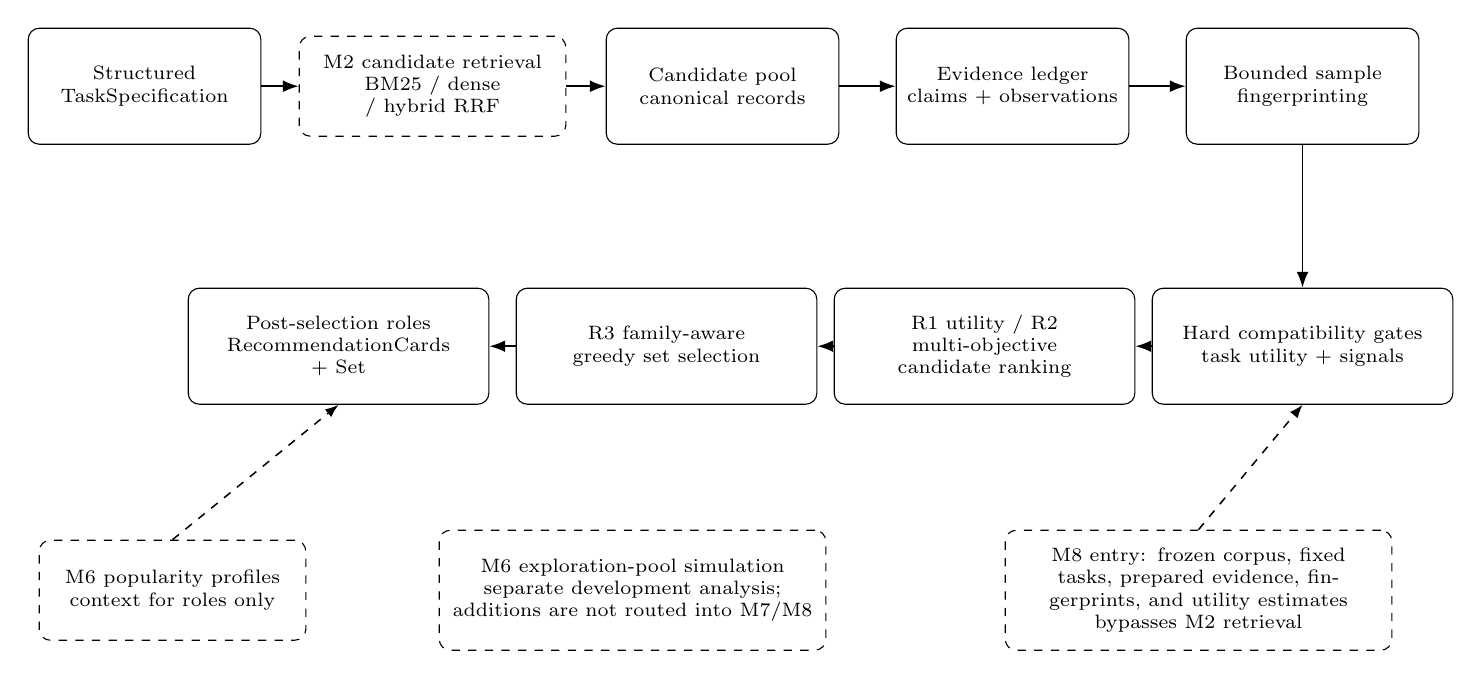
\begin{tikzpicture}[x=1in,y=1in,
  box/.style={draw,rounded corners,align=center,text width=1.08in,minimum height=0.58in,inner sep=3pt,font=\scriptsize},
  widebox/.style={draw,rounded corners,align=center,text width=1.42in,minimum height=0.58in,inner sep=3pt,font=\scriptsize},
  note/.style={draw,dashed,rounded corners,align=center,text width=1.25in,minimum height=0.50in,inner sep=3pt,font=\scriptsize},
  longnote/.style={draw,dashed,rounded corners,align=center,text width=1.85in,minimum height=0.60in,inner sep=3pt,font=\scriptsize},
  flow/.style={-{Latex[length=2mm]},line width=0.65pt},
  context/.style={-{Latex[length=1.7mm]},dashed,line width=0.55pt}]
  \node[box] (task) at (0.58,1.30) {Structured\\TaskSpecification};
  \node[note] (retrieval) at (2.02,1.30) {M2 candidate retrieval\\BM25 / dense / hybrid RRF};
  \node[box] (pool) at (3.47,1.30) {Candidate pool\\canonical records};
  \node[box] (ledger) at (4.92,1.30) {Evidence ledger\\claims + observations};
  \node[box] (finger) at (6.37,1.30) {Bounded sample\\fingerprinting};

  \node[widebox] (gate) at (6.37,0.00) {Hard compatibility gates\\task utility + signals};
  \node[widebox] (rank) at (4.78,0.00) {R1 utility / R2 multi-objective\\candidate ranking};
  \node[widebox] (select) at (3.19,0.00) {R3 family-aware\\greedy set selection};
  \node[widebox] (output) at (1.55,0.00) {Post-selection roles\\RecommendationCards + Set};

  \node[note] (m6profiles) at (0.72,-1.22) {M6 popularity profiles\\context for roles only};
  \node[longnote] (m6sim) at (3.02,-1.22) {M6 exploration-pool simulation\\separate development analysis; additions are not routed into M7/M8};
  \node[longnote] (m8) at (5.85,-1.22) {M8 entry: frozen corpus, fixed tasks, prepared evidence, fingerprints, and utility estimates\\bypasses M2 retrieval};

  \draw[flow] (task.east) -- (retrieval.west);
  \draw[flow] (retrieval.east) -- (pool.west);
  \draw[flow] (pool.east) -- (ledger.west);
  \draw[flow] (ledger.east) -- (finger.west);
  \draw[flow] (finger.south) -- (gate.north);
  \draw[flow] (gate.west) -- (rank.east);
  \draw[flow] (rank.west) -- (select.east);
  \draw[flow] (select.west) -- (output.east);
  \draw[context] (m6profiles.north) -- (output.south);
  \draw[context] (m8.north) -- (gate.south);
\end{tikzpicture}
\caption{Implemented recommendation path and evaluation entry points. M2 retrieval is a candidate-generation component; M8 starts from its frozen candidate corpus and bypasses M2. M6's popularity profiles may supply post-selection role context, while its exploration-pool simulation is separate and does not feed M7 or M8.}
\label{fig:implemented-pipeline}
\end{figure*}

\section{Implemented Recommendation Pipeline}
\subsection{Candidate Retrieval}
The repository implements BM25 retrieval over canonicalized dataset descriptions, an optional dense retrieval path using a pretrained sentence encoder, and reciprocal-rank fusion for a hybrid comparison. These methods provide candidate-generation alternatives; none is presented as a new retrieval algorithm. The four-query M2 comparison measures them as a development component benchmark. In the frozen M8 protocol, the candidate corpus is fixed and is passed directly to recommendation ranking, so M8 results do not measure end-to-end retrieval recall.

\subsection{Two-Layer Evidence States and Bounded Fingerprinting}
Source adapters preserve source-specific provenance while producing canonical records. The evidence ledger stores claims from repository metadata, dataset documentation, Croissant metadata, access probes, and content observations. Each entry retains its source, field, procedure, timestamp, and any sample scope. The provisional resolver assigns a separate resolution state across entries; downstream compatibility and ranking use the underlying observations and categorical states rather than a scalar confidence estimate. Consequently, a publisher's license or modality statement remains distinguishable from a value directly observed in a bounded probe, and disagreement remains explicit.

When the source and policy permit sample access, the fingerprinting pipeline reads no more than 32 records or 64 MiB and records sample-scoped structural and quality diagnostics. It preserves outcomes such as unsupported access, operational failure, and unknown fields as distinct states. A fingerprint describes only the acquired slice: for example, a single-class result in a 32-row sample is not treated as a full-dataset label-distribution fact. Fingerprints feed the quality and coverage signals but are not themselves utility estimates.

\subsection{Hard Compatibility Gating and Utility Estimation}
The utility estimator checks the three hard constraints defined in Section III before aggregating its seven soft components. A modality gate requires explicit evidence of incompatibility; an unknown modality is not treated as a confirmed mismatch. The governance gate compares the task's prohibited-license constraints with the recorded license claim. The access gate excludes a credential-gated Kaggle candidate when the task requires anonymous public access and does not permit gated access. Gating sets utility to zero and the recommendation engine removes that candidate before scoring the eligible pool.

For candidates that pass these checks, the component scores express heuristic compatibility with the structured task. Their equal-weight mean provides $U(q,d)$. M5 compares configurations against a human-authored reference rubric; this is a development comparison, not independent downstream-model ground truth. The ranking pipeline also carries each component's epistemic state into evidence-support and risk features so that unresolved conflicts, failed probes, or sample-limited inferences remain visible to later scoring and card explanations.

\subsection{Multi-Objective Ranking and Family-Aware Greedy Selection}
R1 ranks eligible candidates by composite utility alone. R2 orders them by Eq.~\ref{eq:multiobjective-score}. R3 uses the same intrinsic score within the bounded greedy set selector and adds a set-relative diversity term while enforcing confirmed same-family exclusion. The selectors use deterministic identifier-based tie-breaking. Diversity reflects lineage, schema-token, and source differences; it is a recommendation-set heuristic rather than a guarantee of semantic coverage.

Popularity is retained as contextual information for exposure analysis and post-selection role assignment, but it is excluded from the candidate scoring formula. The separate M6 exploration-pool simulation examined whether under-observed candidates might be surfaced; that simulated pool is not automatically routed into M7 ranking or the M8 benchmark. The ranking and exploration findings therefore remain separate evidence streams.

\subsection{Recommendation Cards and Provenance}
After selection, the engine assigns recommendation roles and creates an immutable card for each chosen dataset. Cards contain dataset and task identifiers, rank and candidate score, component signals, utility-estimate and fingerprint identifiers, evidence-entry identifiers, marginal diversity, and structured explanations for fit, caveats, and placement. Operational context can include source and access or governance claims and a popularity stratum. The accompanying recommendation-set record preserves selected IDs, set-level utility and diversity summaries, gate exclusions, target size, and diversification parameter. This output structure makes a recommendation auditable against its supporting records without converting unresolved evidence into certainty.

\section{Experimental Methodology}
\subsection{Compute Envelope and Development Corpus}
M0 established the local design envelope before downstream experiments: the recorded peak RSS was 37{,}994{,}496 bytes, from which the project derived a 128~MiB process ceiling and a 20{,}000~ms cold per-task budget. Bounded content probes were limited to 32 records and 64~MiB per dataset. These are design limits, not measures of web-scale capacity.

M1--M7 development experiments use a ten-record canonical corpus assembled from Hugging Face, OpenML, UCI, and Kaggle. M2 uses four manually curated queries and five relevance pairs derived from the records' source descriptions. M3--M4 characterize ledger and sample observations on that corpus; M5 evaluates four structured tasks against a human-authored reference rubric; M6 simulates exploration-pool additions for four queries; and M7 compares recommendation sets for four tasks. Their units and data are milestone-specific. None is treated as a sample of the full dataset catalog.

\subsection{Frozen M8 Corpus and Protocol}
M8 evaluates a frozen corpus of 24 dataset records against eight structured tasks, giving 192 task--dataset pairs. The evaluation fixes the target set size at $k=3$, uses seed 20260902, and runs offline with network egress forbidden. The benchmark sends its fixed candidates directly to the recommendation engine; it does not measure retrieval recall. The recorded run is a single deterministic execution on macOS arm64 with Python 3.14.6. Development results and M8 results are therefore reported separately.

Table~\ref{tab:eval-protocol} summarizes the evaluation strata. The four corruption suites operate on fresh copies of benchmark records; the sensitivity sweep changes configured scoring weights and diversification strength without refitting them. M8 also includes an internal pipeline-consistency audit of M7 scores against a rubric related to M5; it is not an external validation set.

\begin{table*}[t]
\caption{Evaluation Strata and Protocol Boundaries}
\label{tab:eval-protocol}
\centering
\footnotesize
\begin{tabularx}{\textwidth}{p{0.78in}p{1.35in}X p{1.70in}}
\toprule
Setting & Corpus and task scope & Protocol & Resource and evidence boundary \\
\midrule
M0 envelope & Local process measurements & Cold-request and sample-access measurement used to derive the design ceilings & 128~MiB process ceiling; 20{,}000~ms cold per-task budget; 32 records / 64~MiB per sample \\
M2--M7 development & 10 canonical records; four queries or tasks, as specified per milestone & Component-specific retrieval, ledger, fingerprint, rubric, exploration, and ranking experiments & Cached development evidence; M5 labels are human-authored rubric judgments, not independent ground truth \\
M8 frozen benchmark & 24 records $\times$ eight structured tasks = 192 pairs; target $k=3$ & Fixed candidate corpus, deterministic run, seed 20260902; robustness and sensitivity fixtures run separately & Zero egress verified; one recorded macOS arm64 / Python 3.14.6 run; no web-scale or downstream-model evaluation \\
\bottomrule
\end{tabularx}
\end{table*}

\subsection{Baselines, Metrics, and Hypotheses}
M2 compares BM25, MiniLM dense retrieval, and reciprocal-rank fusion using Recall@1 and Recall@3, query latency, model/index-build time, embedding-generation time, and measured process RSS. Because the four-query relevance set is small and metadata-derived, comparisons are descriptive. M5 compares Baselines A (metadata-only), B (metadata plus M3 evidence), and C (metadata, evidence, and M4 fingerprints) using mean Spearman rank correlation against the development rubric, NDCG at 3/5/10, hard-gate counts, and runtime. The rubric was authored for the project and is not independent ground truth.

M7 compares R1 utility-only ranking, R2 multi-objective ranking, and R3 family-aware greedy selection by mean set utility, mean pairwise attribute diversity, and same-family redundancy. M8 reports a nine-rung cumulative ablation using mean set utility, plus the registered H1--H5 outcomes. H1 tests redundancy elimination only where the R1 top-$k$ set contains a qualifying same-family pair; H2 reports evidence-related pair reordering descriptively; H3 applies the preregistered utility-retention tolerance $\epsilon=0.03$; H4 separates the architectural popularity exclusion from an empirical association test; and H5 checks recommendation-role grounding. No inferential significance test is used for these milestone comparisons.

For each M8 task and ablation rung, set utility is the arithmetic mean of composite utility across selected candidates; the reported rung value is the unweighted mean of the eight task-level set means. Rungs 0--3 selected three candidates for every task. After hard gating (Rungs 4--8), four tasks had two selected candidates and four had three. The post-gating changes therefore reflect both candidate eligibility and set composition/size; they are descriptive comparisons, not a matched-size estimate of the gate's isolated effect.

\subsection{Robustness, Sensitivity, and Human Pilot}
The M8 robustness harness evaluates four fixture-based corruptions: metadata omission, injected license conflicts, modality corruption, and endpoint failures. Across ten severity trials it records crashes, evidence-state transitions, hard-gating recall, utility change, and set Jaccard overlap. These are controlled perturbations of the frozen records, not field reliability trials.

Sensitivity analysis perturbs the four positive scoring weights within $\pm20\%$, varies the risk weight over 0.12/0.15/0.18, and sweeps $\lambda_{\mathrm{div}}$ from 0.00 to 0.40. Mean recommendation-set Jaccard and Kendall rank correlation are reported relative to the default configuration. The M8 internal pipeline-consistency audit of M7 scores reports Brier and five-bin ECE over 192 rubric-labeled pairs, with a positive-label ratio of 0.09375. These are descriptive internal-consistency diagnostics against a rubric related to M5 utility; they are not calibration estimates.

The human pilot compares minimal cards (Format A) with evidence-augmented cards (Format B) on trust, understanding, and actionability using five-point ratings. Its primary sample contains three participants, each rating seven comparisons: 42 card-level observations and 126 Likert values. We report format means, medians, and paired B-minus-A descriptive differences only. There are no inferential tests. All participants used the same RATER\_1 schedule, so order was not counterbalanced; one participant was an author of the study.

\section{Results}
\subsection{Retrieval and Resource Trade-Off}
On the ten-record, four-query M2 development benchmark, BM25, dense retrieval, and hybrid RRF all achieved Recall@1 of 0.875 and Recall@3 of 1.000. The benchmark therefore did not distinguish retrieval quality among these methods. BM25 mean query latency was 0.0602~ms; dense and hybrid means were 700.1929~ms and 15.0808~ms, respectively. MiniLM index construction took 81{,}000.40~ms and embedding generation 5{,}038.56~ms. The dense model/index run reached 453.22~MiB peak RSS, exceeding the 128~MiB M0 ceiling. BM25's peak RSS was not separately recorded, so no independent memory value is assigned to it. Relevance judgments came from source descriptions; saturation on this small set is not evidence of general retrieval effectiveness.

\begin{table*}[t]
\caption{M2--M7 Development-Corpus Results}
\label{tab:development-results}
\centering
\footnotesize
\begin{tabularx}{\textwidth}{p{0.42in}p{0.90in}X p{1.45in}}
\toprule
Stage & Evaluation scope & Observed result & Evidence boundary \\
\midrule
M2 & 10 records; four queries & Recall@1 0.875 and Recall@3 1.000 for all methods; mean latency BM25 0.0602~ms, dense 700.1929~ms, hybrid 15.0808~ms; dense index build 81{,}000.40~ms, embeddings 5{,}038.56~ms, peak RSS 453.22~MiB & Five metadata-derived relevance pairs; BM25 RSS not separately recorded \\
M3 & 10 records & 107 ledger entries: 54 metadata, 20 access, 13 Croissant, 10 documentation, 10 content; 67 single-source claims (62.6\%); 90/106 unresolved resolutions and one conflict & Ledger composition, not evidence of dataset quality \\
M4 & 10 records; seven sample-evaluated & Runtime 9.31~ms; peak RSS 24.20~MiB; two constant columns; observed-sample null and duplicate rates 0; Rotten Tomatoes first 32 rows had majority-label ratio 1.0 & Beans sample endpoint returned HTTP 502; two Kaggle samples were unsupported; findings are sample-scoped \\
M5 & Four tasks $\times$ 10 records; 120 baseline evaluations & Mean Spearman A/B/C = 0.9576/0.9576/0.9667 ($\Delta=+0.0091$); NDCG@3/5/10 = 0.5421/0.6094/0.6766 for all; 90/120 hard-gated (75.0\%); 25.00~MiB, 26.06~ms & Human-authored reference rubric; no independent downstream-performance target \\
M6 & Four development queries & Five of ten popularity profiles were under-observed; measured strata: two very-high, one high, one low, one very-low. Two under-observed high-utility candidates were added only for $q_{\mathrm{tabular\_wine}}$; pool utility 0.5476$\to$0.6857; zero strict hidden gems & Exploratory development simulation; the other three queries had no additions \\
M7 & Four tasks; 12 sets & R1/R2: utility 0.8506, diversity 0.5278, redundancy 1; R3: utility 0.8536, diversity 0.5000, redundancy 0; Iris-task utility 0.8809$\to$0.8928; $\lambda_{\mathrm{div}}=0.20$ & One development mirror pair; metrics describe this corpus and realized set sizes \\
\bottomrule
\end{tabularx}
\end{table*}

\subsection{Evidence and Bounded Content Findings}
M3 recorded 107 entries across ten development records. Single-source claims accounted for 67 entries (62.6\%); resolution remained unresolved for 90 of 106 claim resolutions, with 15 unknown and one conflicting resolution. The conflict was a Rotten Tomatoes license string (`MIT`) versus a Croissant license URI. The ledger retained the differing source claims instead of normalizing them into agreement. Entry counts describe the harvested corpus and do not measure completeness or intrinsic quality.

M4 produced ten fingerprints, of which seven had sample data evaluated. One sample operation failed (Beans, HTTP 502) and two Kaggle sample routes were unsupported under the access policy. Across the evaluated samples, the observed null-cell and duplicate-record rates were both zero; two constant columns were detected. In the first 32 Rotten Tomatoes rows, the observed label was constant and the majority-label ratio was 1.0. This is a property of that bounded slice, not an estimate of the complete dataset's label distribution.

\subsection{Utility Estimation and Hard Gating}
Across the four-task, ten-record M5 development comparison, Baselines A and B had mean Spearman $\rho=0.9576$, while Baseline C reached 0.9667, a descriptive increase of 0.0091. NDCG@3, @5, and @10 were identical across the three configurations at 0.5421, 0.6094, and 0.6766. The rubric comparison thus showed a small rank-correlation change without an observed NDCG change on this corpus. The rubric is human-authored and shares compatibility concepts with the estimator; these numbers are not estimates of model-performance benefit.

Hard gates excluded 90 of 120 task--candidate evaluations (75.0\%), primarily where the task modality and candidate modality were confirmed incompatible. M5 used 25.00~MiB peak RSS and 26.06~ms across the 120 evaluations. Neither the gate count nor its resource cost implies that uncertain candidates were judged unsuitable: unknown evidence remained distinct from confirmed incompatibility.

\subsection{Long-Tail Exploration and Development Diversification}
M6 profiled ten records: popularity was measured for five (two very-high, one high, one low, one very-low), while five remained under-observed. Across four development queries, the exploration simulation added two under-observed high-utility candidates only for $q_{\mathrm{tabular\_wine}}$; its candidate-pool mean utility rose from 0.5476 to 0.6857. The other three queries had no additions, and no candidate met the strict hidden-gem rule. This is an exploratory result on the ten-record development corpus, not evidence of web-scale long-tail discovery.

M7's R1 and R2 sets each had mean utility 0.8506, mean attribute diversity 0.5278, and one same-family redundant pair. R3's family check removed that observed Iris mirror pair; mean set utility was 0.8536 and redundancy was zero. On the Iris task, mean set utility changed from 0.8809 to 0.8928. The aggregate diversity statistic was 0.5000 for R3 versus 0.5278 for R1/R2; therefore, these results support removal of the known family duplicate in this development case, not an increase in the reported diversity metric generally. At revision `bff0767`, M7 recorded 25.88~MiB peak RSS and 13.66~ms total for 12 sets (about 1.14~ms/set by division).

\subsection{Frozen Benchmark, Ablation, and H1--H5}
The M8 frozen run evaluated 24 dataset records against eight tasks (192 task--dataset pairs), with target $k=3$. It completed in 327.49~ms at 33.11~MiB peak RSS, and zero egress was verified. The cumulative ablation's mean set utility rose from 0.2191 for corpus order to 0.8189 after hard gating and 0.8588 at the utility-only rung; later multi-objective, farthest-first, and full-system rungs each remained at 0.8588. The BM25, dense, and hybrid retrieval rungs were not a retrieval-recall evaluation here: their output was converted to candidate ordering within a fixed corpus. These cumulative comparisons do not isolate every component's general contribution.

The registered outcomes have different meanings. H1 was N/A: zero tasks had a same-family pair in the R1 top-$k$ set, so there was no qualifying M8 case in which to test elimination. H2 remained exploratory: R2 reordered three of 33 utility-near divergent pairs (9.1\%) across six of eight tasks. H3 met its utility-retention criterion ($\bar U_{R1}=\bar U_{R3}=0.8588$, observed difference 0.0000, tolerance $\epsilon=0.03$), but this equality occurred in a corpus with no qualifying mirror case and does not show that diversification improved M8 utility. H4 was supported as an architectural invariant because popularity counters are excluded from scoring; the empirical per-task association was N/A for all eight tasks because measured popularity values were insufficient or constant. H5 was supported: all 20 of 20 assigned roles met their grounding preconditions, with zero violations.

\begin{table}[t]
\caption{M8 Cumulative Ablation}
\label{tab:m8-ablation}
\centering
\footnotesize
\begin{tabular}{clc}
\toprule
Rung & Candidate path & Mean set utility \\
\midrule
0 & Corpus order & 0.2191 \\
1 & BM25 only & 0.4684 \\
2 & Dense only & 0.4085 \\
3 & Hybrid RRF & 0.4414 \\
4 & Hybrid plus hard gating & 0.8189 \\
5 & Utility only (R1) & 0.8588 \\
6 & Multi-objective (R2) & 0.8588 \\
7 & Farthest-first without family check & 0.8588 \\
8 & Full system (R3) & 0.8588 \\
\bottomrule
\end{tabular}
\end{table}

\begin{table*}[t]
\caption{M8 Registered Hypothesis Outcomes}
\label{tab:m8-hypotheses}
\centering
\footnotesize
\begin{tabularx}{\textwidth}{p{0.45in}p{0.85in}X p{2.00in}}
\toprule
Hyp. & Status & Observed outcome & Interpretation boundary \\
\midrule
H1 & N/A & Zero qualifying R1 sets contained a same-family pair & No M8 case exercised the redundancy-elimination criterion \\
H2 & Exploratory & 3 of 33 divergent pairs reordered (9.1\%); pairs spanned 6/8 tasks & Descriptive frequency; not a general disambiguation rate \\
H3 & Criterion met & R1 and R3 mean set utility both 0.8588; $\Delta=0.0000$, $\epsilon=0.03$ & Retention under this corpus geometry; no qualifying mirror case to exercise diversification \\
H4 & Supported as invariant & Popularity excluded from scoring; association test N/A in all eight tasks ($n<3$ or constant) & Architectural verification, not an empirical neutrality estimate \\
H5 & Supported & 20/20 roles grounded; zero violations & Result is limited to the roles and cards evaluated in M8 \\
\bottomrule
\end{tabularx}
\end{table*}

\subsection{Robustness and Sensitivity}
The four robustness suites completed ten trials with zero crashes. Metadata omission produced zero evidence-state transitions across its three severities. License-conflict injection produced 16 transitions at each of two severities. Under modality corruption, hard-gating recall was 0.6667 and set Jaccard overlap 0.9375 at both severities. Endpoint-failure fixtures produced 16/40/40 state transitions across three severities, mean utility changes from $-0.00415$ to $-0.00475$, and Jaccard overlap 0.9375. These controlled fixture outcomes characterize the tested perturbations, not all operational failures.

For the registered positive-weight perturbations within $\pm20\%$ and risk weights 0.12, 0.15, and 0.18, aggregate mean Jaccard and Kendall $\tau$ were both 1.0. In the $\lambda_{\mathrm{div}}$ sweep, mean Jaccard relative to default was 1.0 at 0.15 and 0.20, and 0.8125 at 0.30 and 0.40; this finite sweep does not establish stability outside the tested values.

The internal consistency audit used 192 rubric-labeled pairs, 18 positive labels (ratio 0.09375), and reported Brier 0.259314 and five-bin ECE 0.428503. Because the labels came from the M5-related design rubric, these are consistency diagnostics only, not calibration results.

\begin{table*}[t]
\caption{M8 Robustness, Sensitivity, and Internal Consistency Diagnostics}
\label{tab:m8-stability}
\centering
\footnotesize
\begin{tabularx}{\textwidth}{@{}p{1.10in}p{0.90in}X p{1.85in}@{}}
\toprule
Protocol & Cases & Selected outcomes & Evidence boundary \\
\midrule
Metadata omission & 3 severities & 0 state transitions; zero crashes & Corruption fixtures only \\
License conflict & 2 severities & 16 state transitions per severity; zero crashes & Injected claim conflicts; no legal resolution \\
Modality corruption & 2 severities & Gating recall 0.6667; set Jaccard 0.9375; zero crashes & Fixture-specific gating behavior \\
Endpoint failure & 3 severities & 16/40/40 transitions; utility $\Delta$ from $-0.00415$ to $-0.00475$; Jaccard 0.9375 & Simulated access failures \\
Positive/risk weights & $\pm20\%$ positive weights; risk 0.12/0.15/0.18 & Mean Jaccard $=1.0$; mean Kendall $\tau=1.0$ & Tested weight perturbations relative to default \\
$\lambda_{\mathrm{div}}$ sweep & 0.00--0.40 & Jaccard 1.0 at 0.15/0.20; 0.8125 at 0.30/0.40 & Finite parameter sweep \\
Consistency audit & 192 pairs; 18 positive labels & Brier 0.259314; five-bin ECE 0.428503 & Same-family rubric; not independent calibration \\
\bottomrule
\end{tabularx}
\end{table*}

\subsection{Exploratory Human Evaluation}
Across the primary first-exposure ratings, Format B had higher descriptive means than Format A on all three dimensions. The paired mean differences were +1.8095 for trust, +3.1905 for understanding, and +3.0000 for actionability; corresponding medians were +2, +3, and +3. The primary analysis comprises three participants and seven comparisons each, with 21 participant--comparison ratings per format. All three participants completed the same RATER\_1 schedule, so presentation order was not counterbalanced; one participant was an author. No inferential test was conducted, and the ratings do not establish practitioner benefit or generalize beyond this small pilot.

\begin{table}[t]
\caption{Human-Pilot Primary Ratings (Descriptive)}
\label{tab:human-pilot}
\centering
\footnotesize
\begin{tabularx}{\columnwidth}{p{0.88in}*{3}{>{\centering\arraybackslash}X}}
\toprule
Dimension & A mean (med.) & B mean (med.) & B$-$A mean (med.) \\
\midrule
Trust & 1.9524 (2) & 3.7619 (4) & +1.8095 (+2) \\
Understanding & 1.6190 (2) & 4.8095 (5) & +3.1905 (+3) \\
Actionability & 1.3333 (1) & 4.3333 (4) & +3.0000 (+3) \\
\bottomrule
\end{tabularx}
\end{table}

\section{Discussion}
The results support a bounded account of the system rather than a general comparison of dataset recommenders. In M2, BM25, dense retrieval, and hybrid RRF reached the same Recall@1 and Recall@3 on a small, metadata-derived query set. M8 does not extend that retrieval test: its candidates were fixed before ranking. The M8 ablation's utility metric averages selected-candidate utility within each task's set and then averages equally across eight tasks. Four tasks returned two candidates after gating, so the 0.4414-to-0.8189 change is affected by both eligibility and set size; it is not an isolated gate effect at matched set size. Later utility-only ranking increased the mean to 0.8588, while multi-objective ranking and the two set-selection rungs did not change the aggregate mean. The cumulative stages do not isolate the general causal contribution of each mechanism.

The component studies provide information that the frozen benchmark cannot supply by itself. M3 records how often claims remain single-source or unresolved, and retains a metadata conflict instead of silently normalizing it. M4 shows what the bounded acquisition path can and cannot observe, including a failed endpoint, unsupported routes, and a sample-local constant label. M5 provides a development comparison to a human-authored rubric, while M6 and M7 exercise exploration and family-aware selection on a ten-record corpus. These are distinct forms of evidence: the ledger counts do not measure quality, the M5 rubric is not external ground truth, M6 is exploratory, and M7 contains one observed mirror pair.

The M7 result is correspondingly specific. R3 removed the Iris same-family pair seen under R1/R2 without lowering aggregate set utility in that development comparison. The reported aggregate attribute-diversity value was lower for R3, and M8 contained no qualifying case for H1. This shows that the selector removed the observed development-corpus family duplicate; it does not establish that recommendation diversity generally increased or that diversification improved M8 utility.

The resource results clarify a design trade-off. BM25 retrieval, evidence handling, fingerprinting, utility estimation, and ranking were measured as separate components or development runs within the M0-derived local envelope; M8 separately measured fixed-corpus recommendation. The optional MiniLM dense path exceeded both the memory ceiling and the cold build-time budget, so the retrieval-quality parity on the small M2 corpus does not offset that measured cost under the stated envelope. M8 itself completed offline within the memory ceiling on one recorded environment. These results show feasibility for the measured runs, not a resource guarantee across machines or larger corpora.

In this pilot, Format B received higher descriptive mean ratings than Format A on trust, understanding, and actionability. The study measured ratings on seven selected comparisons, not choices in a real workflow, decision quality, or practitioner benefit. With three participants, a shared presentation schedule, and one author-participant, its role is descriptive and hypothesis-generating only.

\section{Limitations and Threats to Validity}
The retrieval evidence is limited to four queries, ten records, and five relevance pairs derived from source descriptions. All three M2 methods saturated Recall@3, so these measurements cannot establish relative retrieval effectiveness on a larger or more varied catalog. The development corpus contains ten records; M3--M7 findings describe those records and tasks only. M6 is an exploration-pool simulation, and M7's removal of one same-family pair is a single development-corpus observation.

The M5 reference judgments were human-authored for the project and share compatibility concepts with the utility estimator. M8's pipeline-consistency audit uses a related rubric, so its Brier and ECE values are not independent calibration measures. H4's architectural invariant—that popularity is excluded from candidate scoring—was verified, but its empirical per-task association was not estimable because each task had fewer than three measured popularity points or a constant value. H1 was N/A: no M8 task had a qualifying same-family pair in its R1 top-$k$ set. H3's equal mean utility therefore represents retention under the realized candidate geometry, not an exercised diversification benefit.

The frozen M8 benchmark covers 24 records and eight structured tasks, with zero network egress during one deterministic run. It is not web-scale validation, cross-machine replication, or a downstream-model evaluation. No model was trained to test whether the recommended datasets improve predictive performance. The input is a structured task specification rather than a natural-language request, and the ranking weights and utility components are fixed heuristics rather than learned parameters.

Content verification is bounded to at most 32 records and 64~MiB per dataset. Sample diagnostics can reflect slice ordering or endpoint behavior and must not be generalized to complete datasets. Some sample routes were unsupported under the access policy, and the Beans sample request failed with HTTP 502. Missing, failed, and unsupported evidence remains visible, but it also limits how much of each candidate can be verified.

The M6 findings are exploratory, and the human pilot is small and descriptive: three participants rated seven comparisons each; all used the same RATER\_1 order schedule, counterbalancing was not realized, and one participant was an author. The evaluation therefore cannot estimate broad user benefit. Finally, M7's resource figures are taken from the specified `bff0767` artifact and its results note (25.88~MiB and 13.66~ms). A modified worktree copy of \texttt{m7\_summary.json} reports 25.67~MiB and 17.23~ms. This artifact discrepancy remains unresolved; the paper consistently reports the requested revision's figures rather than mixing the two versions.

\section{Conclusion}
This work implemented a local-first dataset recommendation pipeline that combines structured task constraints, source-attributed evidence states, bounded sample fingerprints, hard compatibility gates, heuristic utility, family-aware set selection, and provenance-linked recommendation cards. On the evaluated development corpus, the pipeline recorded unresolved and conflicting evidence, preserved sample-access failures, and removed one observed same-family duplicate in M7. On the frozen 24-record, eight-task M8 benchmark, it completed offline within the M0 memory ceiling; its cumulative ablation reached mean set utility 0.8588, while the benchmark did not contain a qualifying case to test H1's redundancy criterion.

The contribution is the implemented integration and its scoped evaluation under a measured local resource envelope. The results do not establish web-scale recommendation effectiveness, downstream model improvement, calibrated suitability scores, or practitioner benefit. Larger and more varied corpora, independent suitability judgments, downstream-task evaluation, and replicated user studies remain necessary to establish those outcomes.

% The built-in single-file editor compiler does not run BibTeX or import
% sibling .bib files. Keep references.bib as the maintained source and mirror
% its verified entries here so the live editor preview has resolved citations.
\begin{thebibliography}{8}
\bibitem{noy2019googledatasetsearch}
N.~F. Noy, M. Burgess, and D. Brickley, ``Google Dataset Search: Building a
search engine for datasets in an open Web ecosystem,'' in \emph{Proc. World
Wide Web Conf.}, 2019, pp. 1365--1375, doi: 10.1145/3308558.3313685.

\bibitem{viswanathan2023datafinder}
V. Viswanathan, L. Gao, T. Wu, P. Liu, and G. Neubig, ``DataFinder:
Scientific dataset recommendation from natural language descriptions,'' in
\emph{Proc. 61st Annu. Meeting Assoc. Comput. Linguistics, vol. 1: Long
Papers}, 2023, pp. 10288--10303, doi: 10.18653/v1/2023.acl-long.573.

\bibitem{mazumder2023dataperf}
M. Mazumder \emph{et al.}, ``DataPerf: Benchmarks for data-centric AI
development,'' in \emph{Advances in Neural Information Processing Systems},
vol. 36, 2023, pp. 5320--5347, doi: 10.52202/075280-0235.

\bibitem{akhtar2024croissant}
M. Akhtar \emph{et al.}, ``Croissant: A metadata format for ML-ready
datasets,'' in \emph{Advances in Neural Information Processing Systems 37,
Datasets and Benchmarks Track}, 2024, pp. 82133--82148, doi:
10.52202/079017-2610.

\bibitem{pushkarna2022datacards}
M. Pushkarna, A. Zaldivar, and O. Kjartansson, ``Data Cards: Purposeful and
transparent dataset documentation for responsible AI,'' in \emph{Proc. 2022
ACM Conf. Fairness, Accountability, and Transparency}, 2022, pp. 1776--1826,
doi: 10.1145/3531146.3533231.

\bibitem{longpre2023dataprovenance}
S. Longpre \emph{et al.}, ``The Data Provenance Initiative: A large scale
audit of dataset licensing and attribution in AI,'' arXiv:2310.16787, 2023.

\bibitem{northcutt2021confident}
C.~G. Northcutt, L. Jiang, and I.~L. Chuang, ``Confident learning: Estimating
uncertainty in dataset labels,'' \emph{J. Artif. Intell. Res.}, vol.~70,
pp. 1373--1411, 2021, doi: 10.1613/jair.1.12125.

\bibitem{fahrbach2025gist}
M. Fahrbach \emph{et al.}, ``GIST: Greedy independent set thresholding for
max-min diversification with submodular utility,'' in \emph{Advances in
Neural Information Processing Systems 38}, 2025, doi: 10.52202/085713-1542.
\end{thebibliography}

\end{document}
